
\documentclass{article}
\usepackage{mathtools, amssymb, amsthm, graphicx,ulem} % imports amsmath
\begin{document}
\sloppy
prvni priklad zadani C

\begin{figure}[h!]
  \centering
  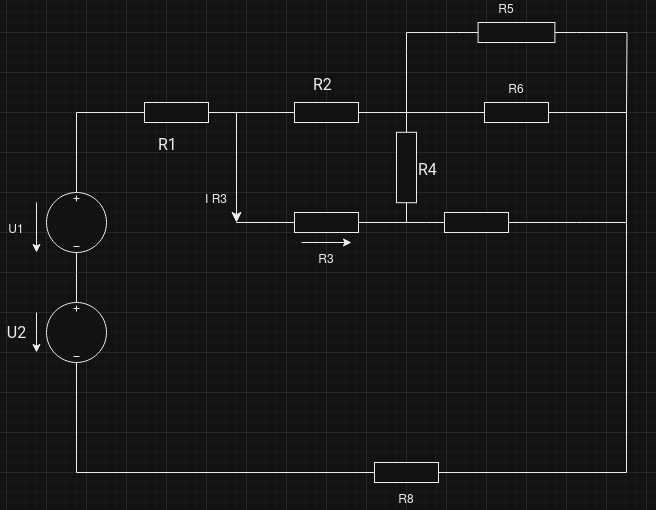
\includegraphics[width=\linewidth, height=0.3\textheight, keepaspectratio]{/home/tjoslef/skola/zapisky/vut/IEL/projekt/uprava_hvezda.drawio.png}
  \caption{Uprava na pomoci hvezdy}
  \label{fig:hvezda}
\end{figure}

\[
    R56 = \frac{R_6 \times R_5}{R_6+ R_5}
\]

\begin{figure}[h!]
  \centering
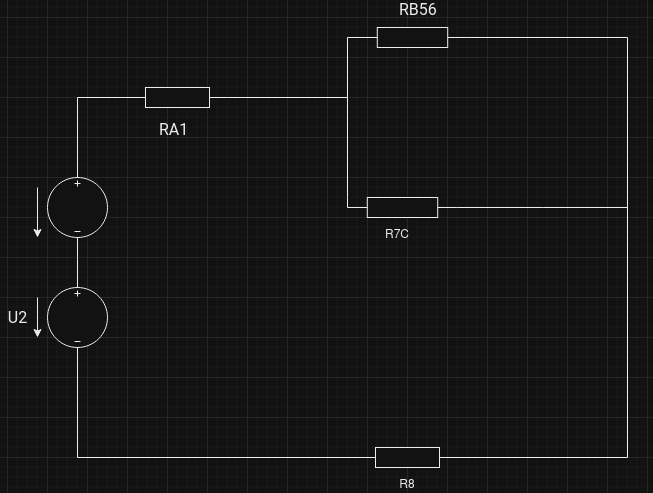
\includegraphics[width=\linewidth, height=0.3\textheight, keepaspectratio]{/home/tjoslef/skola/zapisky/vut/IEL/projekt/dalsi uprava.png}
  \caption{dalsi uprava}
  \label{fig:dalsi_uprava}
\end{figure}

\[
R_{A1} = \frac{R_2 \times R_3}{R_2 + R_3 + R_4} + R_1
\]
\[
R_{A1} = \frac{810 \times 220}{810 + 220 + 190} + 450
\]

\[
R_{B56} = \frac{R_2 \times R_4}{R_2 + R_3 + R_4} +\frac{R_6 \times R_5}{R_6+ R_5}
\]
\[
R_{B56} = \frac{810 \times 220}{810 + 190 + 720} + \frac{220 \times 720}{220+ 720}
= 284.320
\]
\[
R_{C7} = \frac{R_3 \times R_4}{R_2 + R_3 + R_4} + R_7
\]
\[
R_{C7} = \frac{190 \times 220}{810 + 190 + 720} + 260 = 284.302
\]

\[
R = \frac{270.340 \times 284.320}{270.340+284.320}  + 576.148 + 180 \quad \Rightarrow \quad R = 894.770
\]

\[
I = \frac{U}{R} = \frac{180}{894.770} \quad \Rightarrow \quad I = 0.201
\]

\[
U_{R3} = U - U_{R2}
\]
\[
U_{R2} = R_2 \times I
\]
\[
U_{R2} = 810 \times 0.201 = 162.81 \, \text{V}
\]
\[
U_{R3} = 180 - 810 \times 0.201 = 180 - 162.81 = 17.19 \, \text{V}
\]

\[
I_{R3} = \frac{U_{R3}}{R_3}
\]
\[
I_{R3} = \frac{17.19}{190} = 0.0905 \, \text{A}
\]
\end{document}


